\begin{question}
  Justify the relations $y = y'$ and $z = z'$ of Eq1-1a by symmetry arguments.
\end{question}

\begin{solution}
  Eq1-1a describes the Galilean transformation between the two frames of reference depicted in \figref{fig:1q1}.
  \begin{align*}
    x' &= x - vt \\
    y' &= y \\
    z' &= z
  \end{align*}

  The transformation between $y$ and $y'$ because for $y=y_0$, $y'=y_0$ (see red lines in \figref{fig:1q1}). Similarly for $z$ and $z'$.

  \begin{figure} \centering
  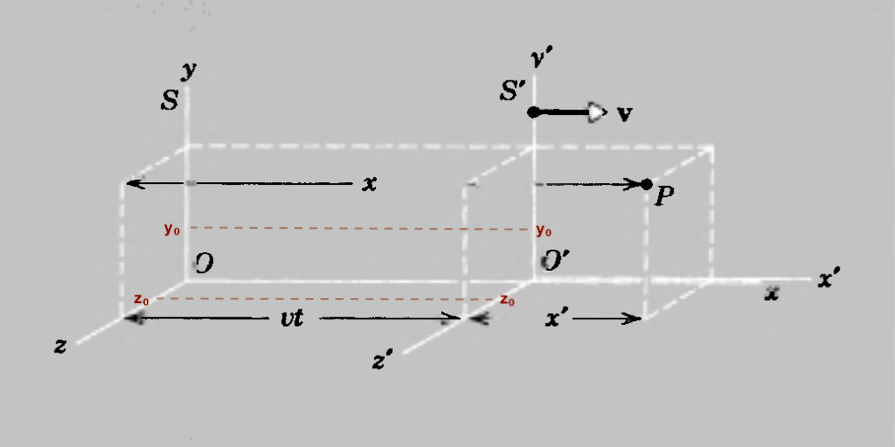
\includegraphics[width=9cm]{fig/1q1.png}
  \caption{Resnick's diagram depicting the two inertial frames of reference $S$ and $S'$. $S'$ is moving with velocity $v$ with respect to $S$. Point $P$ is an event, whose space-time coordinates may be measured by each observer.}\label{fig:1q1}
  \end{figure}
\end{solution}

\begin{question}
  Momentum is conserved in a collision of two objects as measured by an observer on a uniformly moving train. Show that momentum is also conserved for a ground observer.
\end{question}
\begin{solution}
  Consider two point particles of mass $m_1$ \si{kg} and $m_2$ \si{kg} travelling at speeds $v_1$ \si{m.s^{-1}} and $v_2$ \si{m.s^{-1}} respectively (\figref{fig:1q2}). Take the direction of motion of $v_1$ as being the positive direction. Then the total momentum for an observer inside the train before the collision is

  \begin{equation}
    p = m \cdot v, ~ p_{\text{before}} = m_1 v_1 - m_2 v_2
  \end{equation}

  \begin{figure} \centering
    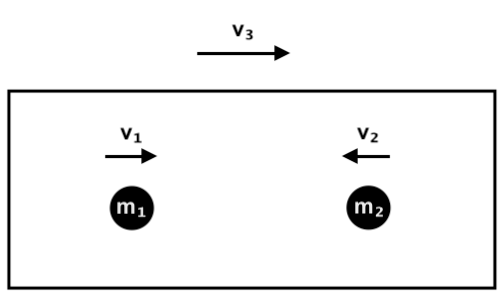
\includegraphics[width=6cm]{fig/1q2.png}
    \caption{Two particles colliding inside a train travelling at velocity $v_3$ \si{m.s^{-1}}.} \label{fig:1q2}
  \end{figure}
\end{solution}
